\documentclass{IEEEtran}

\usepackage{amsmath}
\usepackage{listings}
\lstset{
    basicstyle=\small\ttfamily,
    breaklines=true
}
\usepackage{graphicx}
\graphicspath{ {./images/} }

\title{Readings about Segment Trees}
\author{Diego Linares - kiwiAipom}

\begin{document}
  \maketitle
  \section{Algorithms Live - Segment Trees}
    More of a way of thinking about a problem, rather than a data structure, much like DP.\par 
    Takes the recursion pattern of \textit{MergeSort} and \textit{Divide and Conquer}, and turning it into a data structure.\par
    So you have a \texttt{list} and you cut it in half and now you have 2. Do keep doing this until each list is of size 1. Allows for a nice visual representation of why \textit{MergeSort} is $n\lg{n}$\par 
    \textbf{How do I make it a data structure?} Well, you can see each division as a node. 
    \begin{center}
      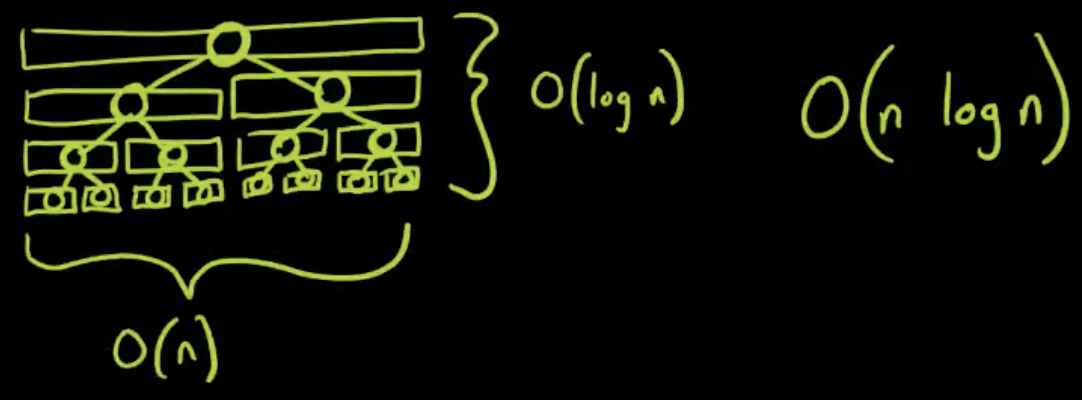
\includegraphics[width=0.40\textwidth]{intoStructure.png}
    \end{center}
    \par Each leaf node is an individual value. And you can push a function (for example: \texttt{min}) upwards through the tree. And I know for each node what particular range is being covered.
    \subsection{Range Minimum Queries (RMQ)}
      Given $[i,j]$ range report the minimum number. \par 
      \textbf{Ex.} Take the case of $[2,7]$. The steps to see:
      \begin{enumerate}
        \item Since $[0,7]$ is not completely covered by $[2,7]$ we go to the left child.
        \item $[0,3]$ is also not completely covered by $[2,7]$ so we go to the left child again.
        \item $[0,1]$ is completely disjoint, so we go back up. And then to the right side.
        \item $[2,3]$ is completely covered by $[2,7]$, so we can return that value.
        \item Unlike a binary search tree, I can go down more than one path, so from the root now I check the right child, and $[4,7]$ is completely covered, so I return that value.
        \item The min of the two will be my answer.
      \end{enumerate}
      \begin{center}
        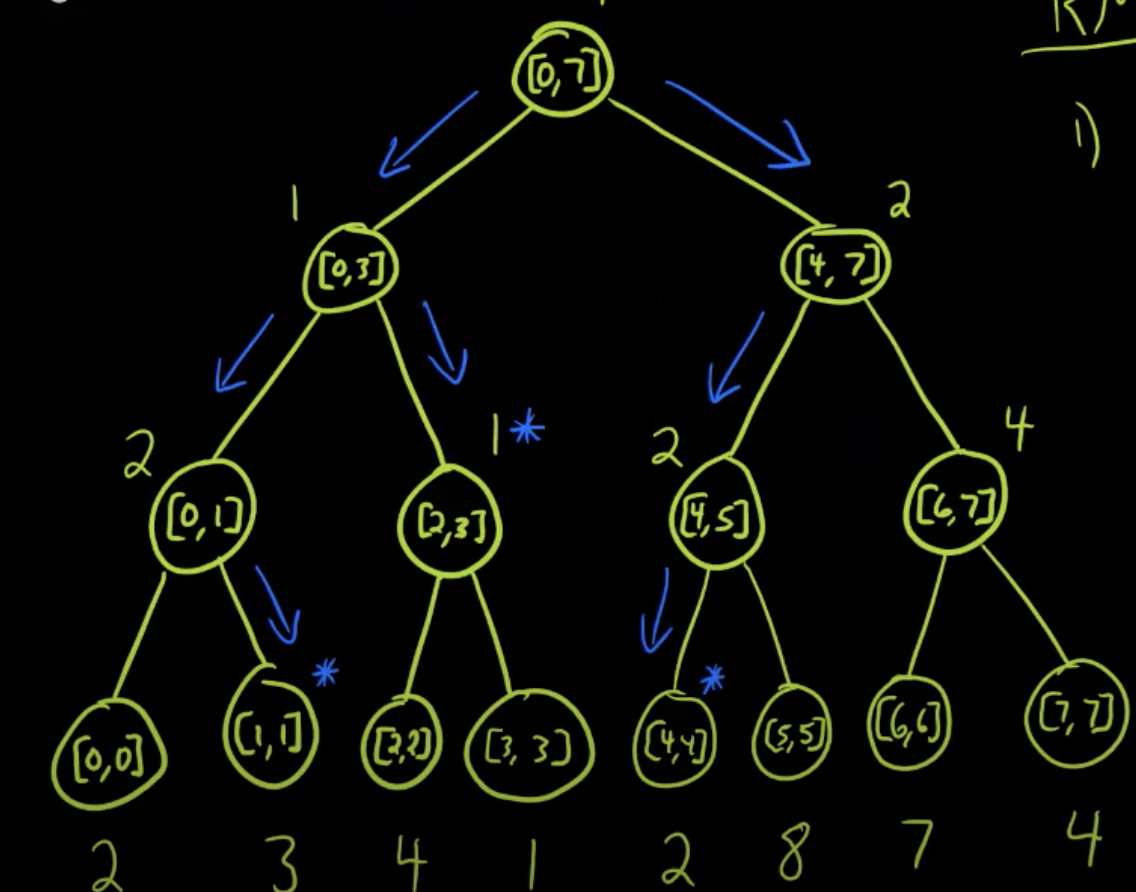
\includegraphics[width=0.30\textwidth]{stExample.png}
      \end{center}
      \par For the \textbf{ex.} $[1,4]$, this time calculate the min of 3 intervals $[1,1],[2,3],[4,4]$, basically, the uppermost segments that are completely covered by the query.\par 
      The execution time, well, the depth of the tree is still $\lg{n}$, but now we are covering more nodes than a regular binary search. But actually, the amount of extra nodes I am covering is a constant factor (at most $1$ node for each one that I find), so the query time is still $\lg{n}$
    \subsection{Lazy Propagation}
      It gives Segment Tree their advantage. Allows to make changes to the sequence by affecting the tree in a "lazy" way.\par 
      \textbf{Ex.} \texttt{increase range [i,j] + val}. But still want to do the queries as a tree.\par 
      \begin{itemize}
        \item Now I don't only store values, but also a change that I want to push down the tree.
        \item We keep track of it in a $\delta$
      \end{itemize}
      
  \section{Simple Approach to Segment Trees 1}
  \section{Simple Approach to Segment Trees 2}
  \section{Bonus: How to Test your Solution on Competitive Programming}
    Useful when you are getting \texttt{Wrong Answer} and you can't find a \textbf{counter-example}.\par 
    First, it is a good idea to write a \texttt{brute}, doesn't matter how slow it is. Try different small tests and compare the results.\par 
    You then could use a \textbf{generator} for small cases. Be sure that your seed is okay so it produces different values. Then you can generate a script to do it multiple times until it differs. An example is:
    \begin{lstlisting}
fo((i=1; i<=100; ++i)) do
  echo $i
  ./gen $i > int
  ./a < int > out1
  ./brute < int > out2
  diff -w out1 out2 || break
done
    \end{lstlisting}
    \par It is recommended that the cases generated are small so the particular pattern is easier to find. If it runs for a while, means that everything works. With \texttt{cat int} you are able to print a countertest.\par 
    If that still doesn't work, \textbf{check for overflows}, since small cases usually don't cover them. \textbf{Edge cases} that should be generated by yourself. Or your array of declaration might be too small. \par
    Some compilation flags that you might use are the following:
    \begin{lstlisting}
g++ -02 std=c++17 -Wno-unused-result -Wshadow -Wall -o a a.cpp
g++ -std=c++17 -Wshadow Wall -o a a.cpp -fsanitize=address -fsanitize=undefined -D_GLIBCXX_DEBUG -g
    \end{lstlisting}
    First oneis for faster runninng time and the second one for checking for mistakes.\par 
    Remember to change the value of the arrays that you are using to a smaller value for small tests. Use \texttt{\#warning} to keep track about it.\par
    \subsection{How to generate trees}
      This is a first script to generate some kind of trees:
      \begin{lstlisting}
srand(atoi(argv[1]));
int n = rand(2,20);
printf("%d\n",n);
for(int i = 2; i <= n; ++i)
{
  printf("%d %d\n", rand(1,i-1), i);
}
      \end{lstlisting}
      \par A smarter way that can generate much more kind of trees is the following. 
      \begin{lstlisting}
vector<pair<int,int>> edges;
for(int i = 2; i <= n; ++i)
  edges.emplace_back(rand(1, i-1),i);
        
vector<int> perm(n+1); // re-naming vertices
for(int i = 1; i <= n; ++i)
  perm[i] = i;
random_shuffle(perm.begin()+1, perm.end());

random_shuffle(edges.begin(), edges.end()); // random order of edges.

for(pair<int,int> edge: edges)
{
  int a = edge.first, b = edge.second;
  if (rand() % 2)
    swap(a,b) // for random order
  printf("%d %d\n",perm[a],perm[b]);
}
      \end{lstlisting}
      \par In the first script, modifying the rand to $(1,1)$ will get you a star, and just putting $i-1$ will get you a line.\par 
      \textbf{Read about proof strings for further info.}
  \begin{thebibliography}{}
    \bibitem{errich}
    \textit{How to test your solution in Competitive Programming, on Linux?},
    Errichto,
    From: https://www.youtube.com/watch?v=JXTVOyQpSGM
  \end{thebibliography}
\end{document}